%
%  $Description: Design and Implementation of Distributed Applications - Project Report$ 
%
%  $Authors: Sara Machado, Rafael Figueiredo, Ricardo Grade$
%  $Date: 2020/12/06$
%
\documentclass[times, 10pt,twocolumn]{article} 
\usepackage{latex8}
\usepackage{times}
\usepackage{graphicx}
\usepackage[font={large}]{caption}
\usepackage[labelfont=bf]{caption}
\graphicspath{{graphs/}}
\setlength{\parskip}{0.14cm}
%------------------------------------------------------------------------- 
\pagestyle{empty}
%------------------------------------------------------------------------- 
\begin{document}

\title{ Design and Implementation of Distributed Applications \\ GStore Project Report}

\author{ 
	Sara Machado \\ 86923
	\and
	Rafael Figueiredo \\ 90770
	\and
	Ricardo Grade \\ 90774
}

\maketitle
\thispagestyle{empty}

\begin{abstract}
	This report explains the implementation of GStore, a distributed Key-Value Pair storage system developed in C\# using gRPC. The objective of this system is to have a high performance while also assuring consistency and availability to its clients. On this Report 2 Versions for this system are presented, the Basic Version, that implements the same consistency that the atomic registers offer, and in the Advanced Version the consistency is relaxed, offering regular registers consistency and additionally does not allow a client to read an older value than it have previously read.
	The performance of both versions is analysed, and the Advanced Version is more efficient in the majority of cases.
\end{abstract}
%------------------------------------------------------------------------- 
\Section{Introduction}
A distributed Key-Value Pair storage system requires a high coordination between all servers of a particular partition. \textbf{GStore} was implemented to provide this coordination, and 2 versions were implemented.

The \textbf{Basic Version}, provides strong consistency and linearizability by implementing atomic registers, but has a single point of failure since write operations rely on the availability of a single server (Master), and a high latency in operations since a lock is required to change a Key-Value Pair. 

The \textbf{Advanced Version} improved the previous version by implementing \textbf{RAFT}  [1], which elects a new Master every time it stops sending proofs of life to the remaining servers on a particular partition, and slightly relaxing the consistency that the \textbf{Basic Version} offers, implementing regular registers while assuring consistency in the readings of values by a client.

The report is organized by firstly explaining in detail each of these versions (Section 2), then it is presented a set of evaluation results that illustrate the performance between both versions on a variety of cases, which are then thoroughly analyzed (Section 3).
%------------------------------------------------------------------------- 
\Section{Proposed Solution}
The System was implemented using \textbf{C\#}, in conjunction with the \textbf{.Net Core} and \textbf{gRPC}.
%------------------------------------------------------------------------- 
\SubSection{Structure}
Each version of the System is organized in 5 modules:  \textbf{Client}, \textbf{GStoreLib}, \textbf{PCS}, \textbf{PuppetMaster} and \textbf{Server}.

In the \textbf{GStoreLib} module, it is implemented all common classes and methods that are used by the other modules.

The \textbf{Client} module implements the mechanisms that allow a client to establish connections to servers, perform operations in the system partitions and receive requests from \textbf{PuppetMaster}.

The \textbf{Server} module implements the mechanisms that allow to receive requests from clients, as well as exchanging messages from other servers, in order to coordinate themselves. It also receives requests from \textbf{PuppetMaster}.

The \textbf{PCS} module is in charge of creating clients and servers processes at the request of the \textbf{PuppetMaster}.

The \textbf{PuppetMaster} module offers a way of controlling the system by a user interface, allowing the creation of new  servers and clients, by making a request to a \textbf{PCS}. This module can also make requests to all nodes of the system to change and check each node status.
%------------------------------------------------------------------------- 
\SubSection{Basic Version}
On this version, it is implemented an atomic register, in order to guarantee high consistency on the clients reads.

\textbf{Writes} can only be done by a single server (Master) in each partition, and are implemented by performing locks on requested objects in all servers of that partition, this allows that while an object is being written, every request to that object is blocked until the write finishes. This way, clients are provided with high consistency and linearizability.

\textbf{Reads}, on the other hand are not required to be performed by the Master, if a read of an object is being done without a concurrent write, it returns right away, otherwise it only receives the response after the write is successfully done, which may cause high delays to the read operations.

\textbf{List Server}, allows a client to see what objects a specific server has in each partition it replicates. This way the clients can verify if all changes it performed were done successfully in a single command.

\textbf{List Global}, allows a client to see all objects of all servers in the system. The implementation of this command is a set of \textbf{List Servers} to all servers, this way a client can verify that all servers of a given partition replicate the written objects.

A client keeps track of which server it was \textbf{last connected} with, and it only changes the server it is attached to if it was requested a command that that server cannot answer. On a \textbf{Read}, the server where it will be performed can be received as an argument, or be randomly chosen in the case that the attached servers does not replicate the requested object. \textbf{Writes} always attach the client to the Master of the object partition.

A client does not make requests to servers that its perfect failure detector already realized that are \textbf{crashed}.

If the Master of a partition \textbf{fails}, no further writes will be performed. Furthermore, if the Master fails while objects are locked, they will be locked forever. In that case, a \textbf{Read} of an object that is locked on all servers of its partition will no longer be performed.
%------------------------------------------------------------------------ 
\SubSection{Advanced Version}
On this version, it is implemented a regular register that additionally does not allow a client read an older value than it have previously read. The algorithm that was followed to implement this version was RAFT [1].

Servers can be found in 3 possible states: \textbf{Follower}, \textbf{Candidate} and \textbf{Master}. There is only a Master in each partition at a time. This grants clients with linearizability on \textbf{Writes}, since that operation can only be performed by servers on this state. The Master is chosen when the system is launched, it periodically (225ms in 225ms) sends heartbeats to its followers which allow them to be sure it is available. A follower has a timer (Between 375ms and 525ms) for each partition it belongs to, that is restarted every time it receives a legitimate heartbeat from that partition Master. In order to be sure that a heartbeat is legitimate each server has a \textbf{Term} for each partition, which indicates how up to date it is on that partition. When a follower times out a new election takes place by incrementing its Term, becoming a candidate, voting for himself and requesting other servers to vote for him. A server votes on a candidate if it has not yet voted on that Term, and its logs are not less up to date than its. A candidate turns himself into a Master if it receives a quorum of votes, sending heartbeats to the followers to take the leadership of that partition. In the case a candidate was not able to get a quorum of votes it restarts its partition timer for a random delay (Between 150ms and 600ms) in order to not turn himself into a candidate at the same time the others do. 

\textbf{Writes}, that are performed by the Master of the partition of the object to be written, generate a log representing it which is immediately appended to the Master logs. However the operation is only concluded when the Master is able to get a quorum of successful updates of the partition servers. When a follower receives a new log from the Master it is appended to the follower stored logs updating itself. For each partition there is a \textbf{Tag} that represents the amount of logs a server has received so far on that partition, that value is sent along with a vote request letting the elector know if the candidate logs are sufficiently updated (\(Candidate.Tag \geq Elector.Tag\)). In the case a Master crashes and has yet to reach a quorum of answers, there could be some inconsistency states among partition servers. If the elected Master did not receive the mentioned update it will erase that log on the other servers in order to leave a system in a consistent state (Rollback). As Masters are dynamically chosen clients can attempt to perform writes on servers that are no longer Masters. In this case the server will let the client know who it believes to be the current Master. If that server is no longer available (Did not answer in 5 seconds) the client will try to perform the write on another server which could be the Master or could redirect him to who it believes to be the current Master.

\textbf{Reads} are done in all servers of the partition of the object to be read, being deemed successfully when it receives a quorum of answers by the partition servers, and it contains an acceptable Tag (\(MaxReceivedTag \geq Client.Tag\)). In the case all available partition servers reply with no acceptable Tag, it will return the client with the value of the most recent one, recovering from a Rollback. When a read is completed the Tag stored in the client is updated with the most recent received Tag.

\textbf{List Server} and \textbf{List Global} are unchanged from the \textbf{Basic Version}.

Similarly to the \textbf{Basic Version} operations on crashed servers are not requested.
%------------------------------------------------------------------------- 
\SubSection{Basic VS Advanced Versions}
Regarding consistency, the \textbf{Advanced Version} implements a slightly more relaxed model in comparison to the \textbf{Basic Version} which offers strong consistency.

Whenever a Master of a given partition becomes unavailable on the \textbf{Basic Version} the \textbf{Writes} will be pending until it becomes available again, or in the case of a crash they will be pending forever. On the \textbf{Advanced Version} this single point of failure does not exist because moments after it becomes unavailable (Temporarily or by Crash) the Followers will time out and elect a new Master for the particular partition. This way the system is still able to perform write operations in the presence of failures on a Master.

The latency of write operations have been significantly decreased on the \textbf{Advanced Version} since locks are no longer required, once atomic registers have been replaced by regular registers. Also on the \textbf{Basic Version} a Master only replies to the client after the update is done in all partition servers, which is no longer needed with the introduction of quorums on the \textbf{Advanced Version} operations.

The latency of read operations are decreased on the \textbf{Advanced Version} in circumstances where they are performed along with write operations. In the best case a quorum of answers is needed for the client to return, while on the \textbf{Basic Version} only a single answer is needed, causing this latency to decrease on a system where no writes are performed.
%------------------------------------------------------------------------- 
\Section{Practical Evaluation}
This system has been analysed in an environment where crashes and freezes can occur. The first 3 scenarios have 3 graphs each, which respectively represent an environment with 20\%, 40\% and 60\% of crashed servers.
%------------------------------------------------------------------------- 
\SubSection{Scenario: System with 5 Servers}
\begin{figure}[h!]
	\centering
	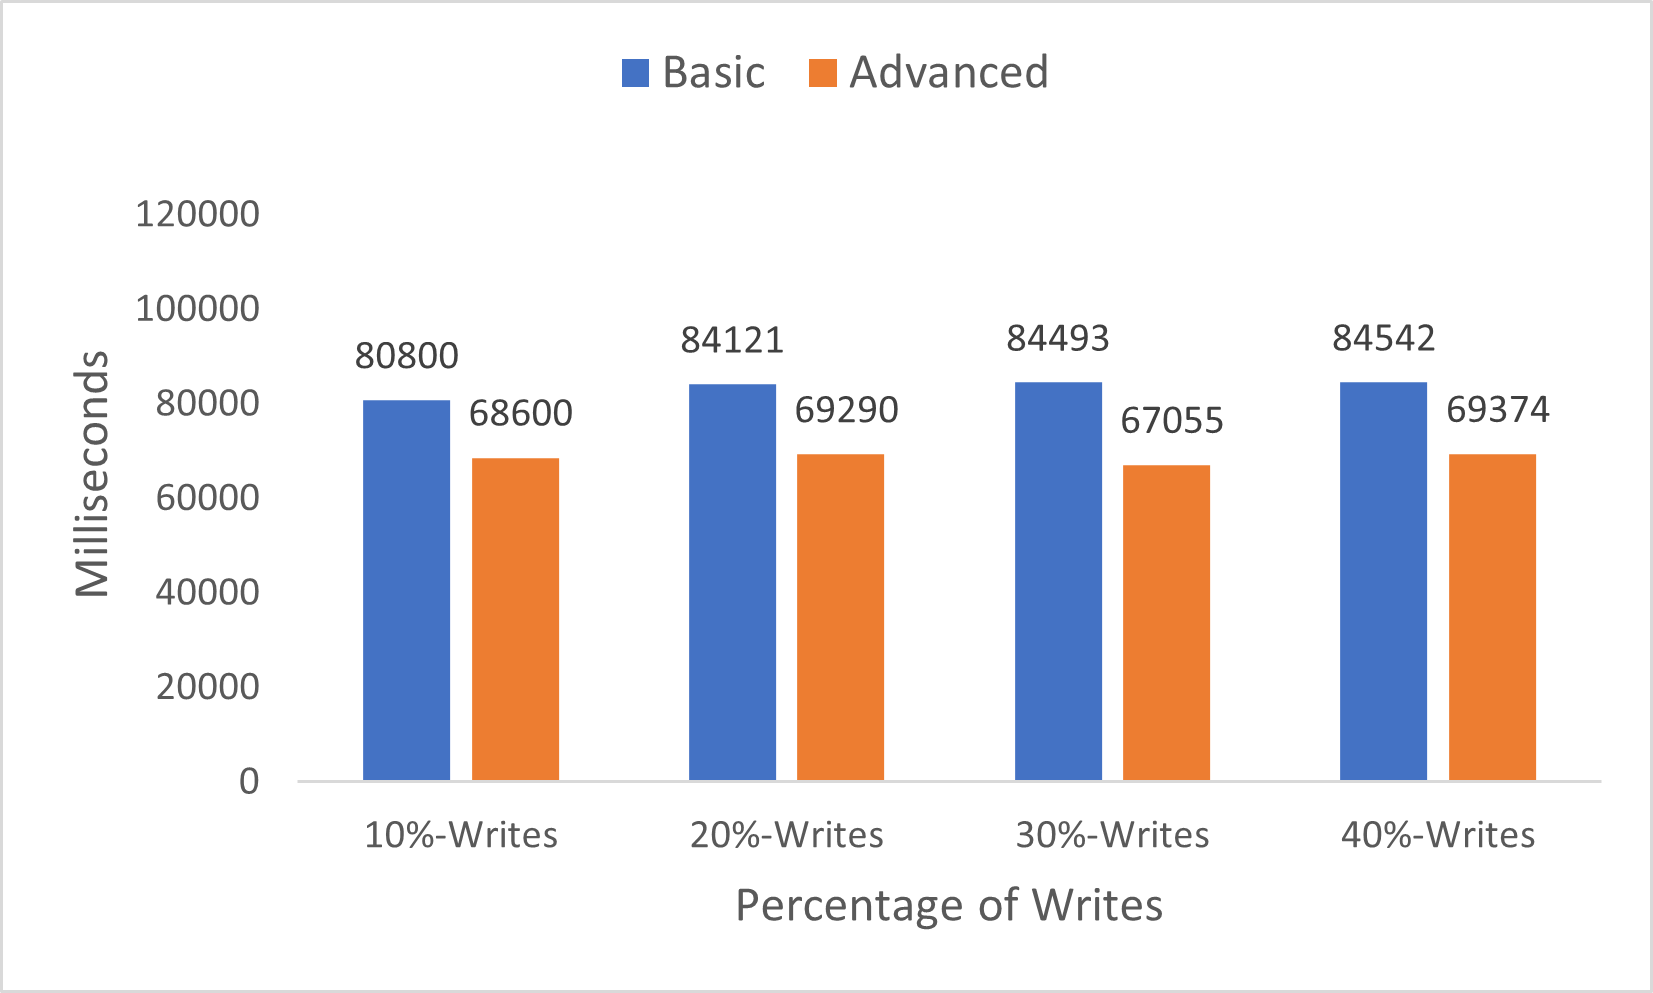
\includegraphics[scale=0.65]{Graphs/Client-5-20.png}
	\caption{Average Time of 10 Clients performing 3000 operations each, on 3 partitions with a total of 5 servers, where 20\% crashed.}
\end{figure}
\newpage
\begin{figure}[h!]
	\centering
	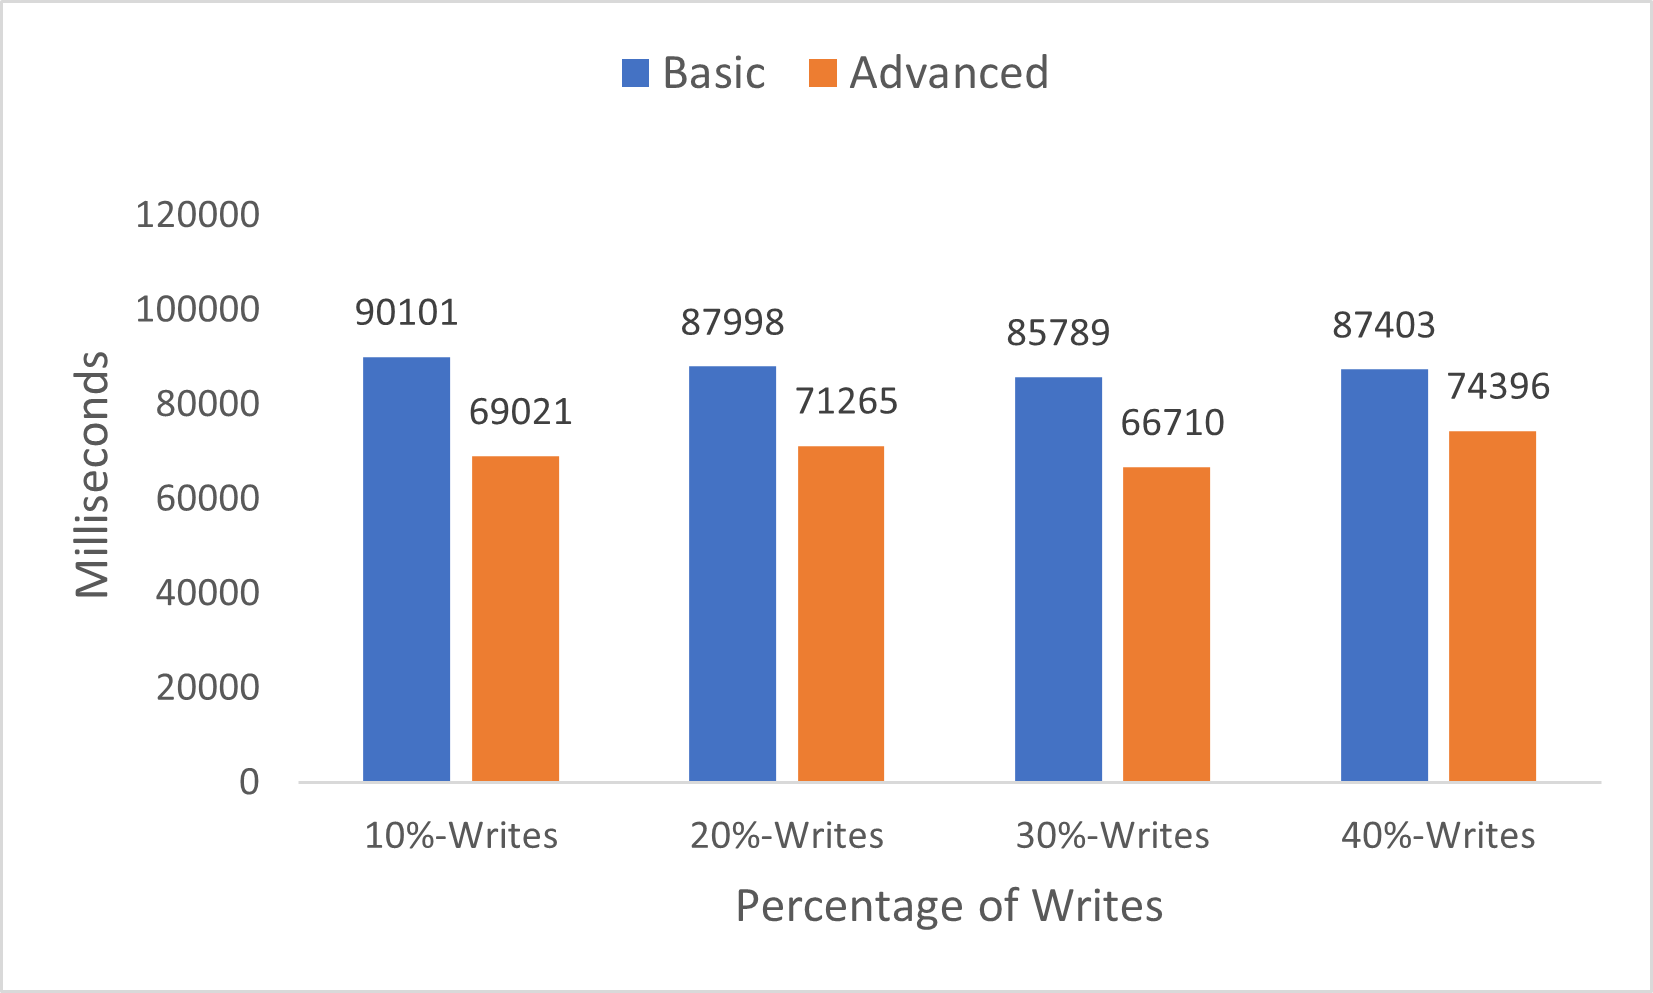
\includegraphics[scale=0.65]{Graphs/Client-5-40.png}
	\caption{Average Time of 10 Clients performing 3000 operations each, on 3 partitions with a total of 5 servers, where 40\% crashed.}
	\vspace{0.15in}
	\centering
	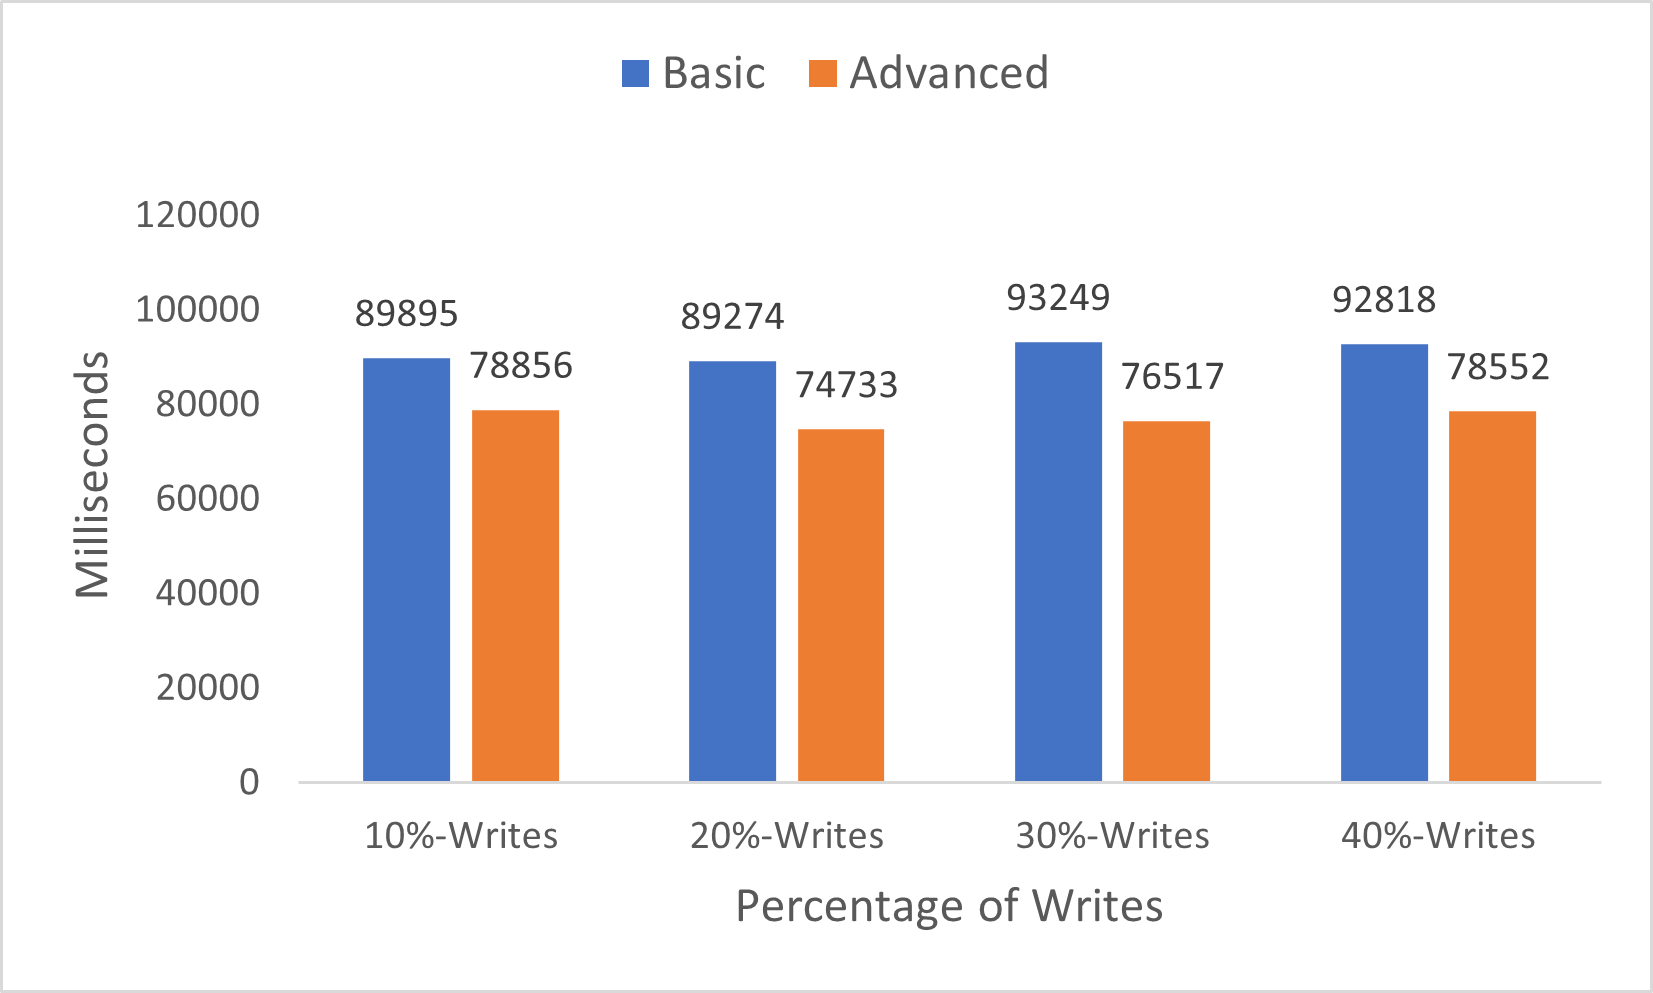
\includegraphics[scale=0.65]{Graphs/Client-5-60.png}
	\caption{Average Time of 10 Clients performing 3000 operations each, on 3 partitions with a total of 5 servers, where 60\% crashed.}
\end{figure}
%------------------------------------------------------------------------- 
\SubSubSection{Discussion of Results}
These graphs illustrate the performance of a system composed by a total of 5 servers on 3 partitions with 3 servers each.

By analyzing the graphs it is possible to observe that the \textbf{Advanced Version} had a better performance than the \textbf{Basic Version} in every single scenario. This happened because although the read operations are predominant, the client script is the same, which will lead, on the \textbf{Basic Version},  to clients delaying each other because of the blocks on objects being written in concurrent operations, which does not happen on the \textbf{Advanced Version}, because the operations do not block each other and can be performed with only a quorum of answers, which in 3000 similar operations will guarantee a better performance overall.
\newpage
%------------------------------------------------------------------------- 
\SubSection{Scenario: System with 10 Servers}
\begin{figure}[h!]
	\centering
	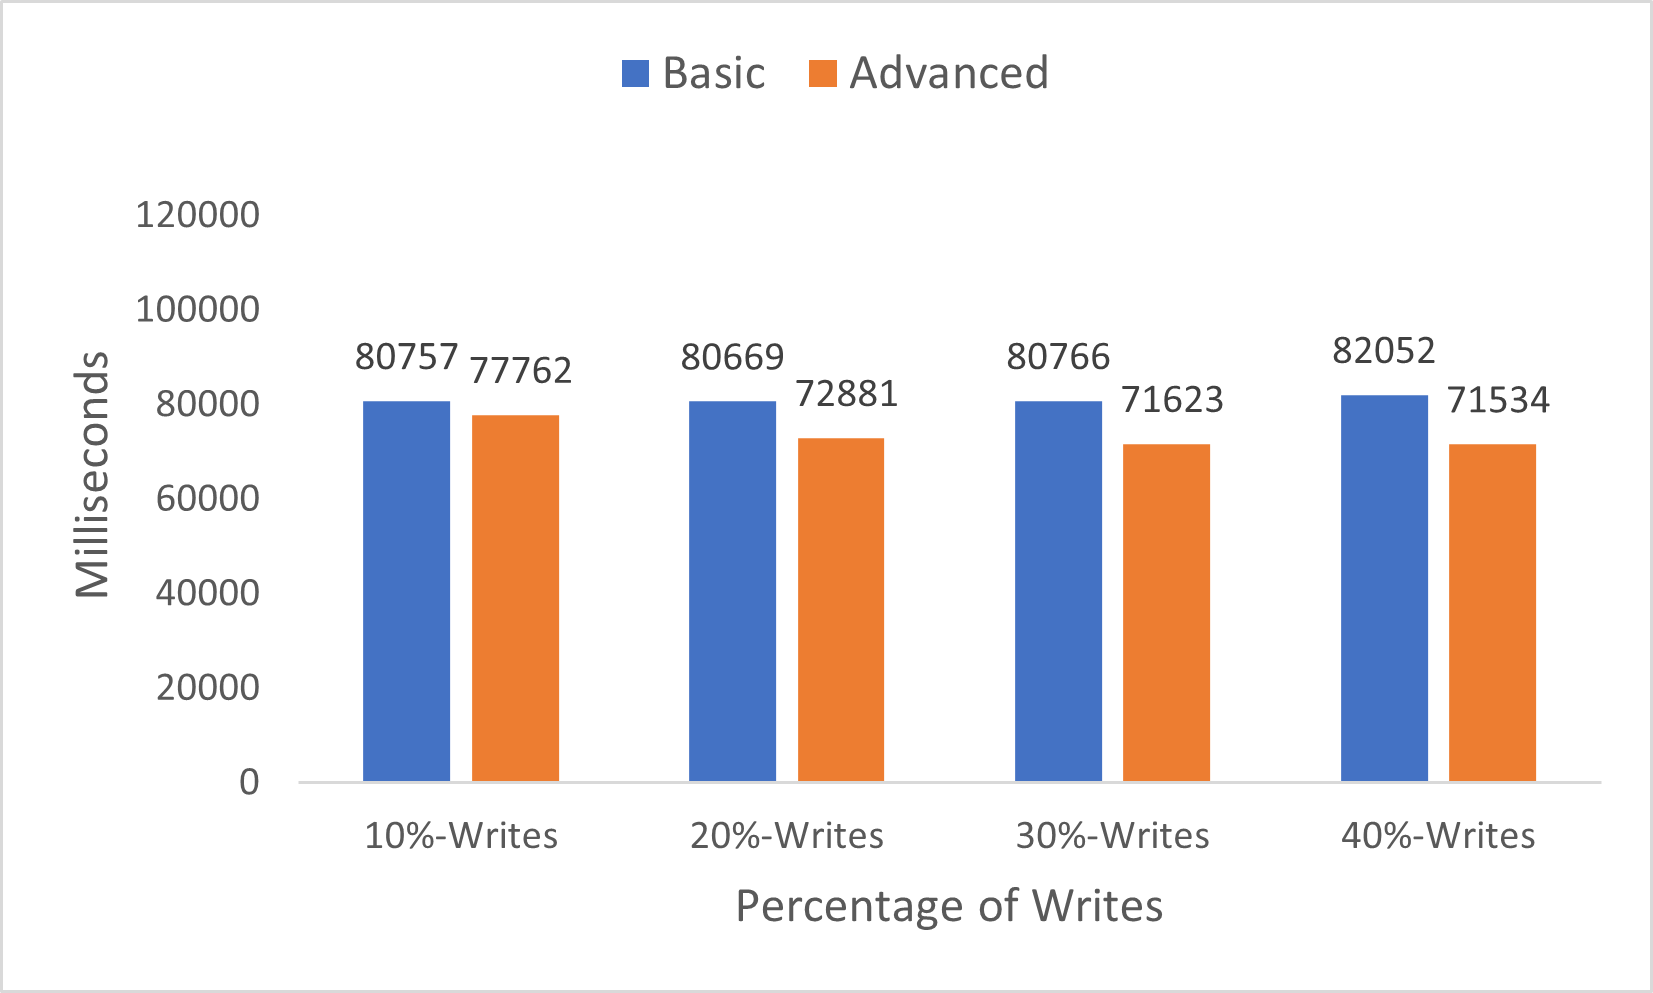
\includegraphics[scale=0.65]{Graphs/Client-10-20.png}
	\caption{Average Time of 10 Clients performing 3000 operations each, on 3 partitions with a total of 10 servers, where 20\% crashed.}
	\vspace{0.15in}
	\centering
	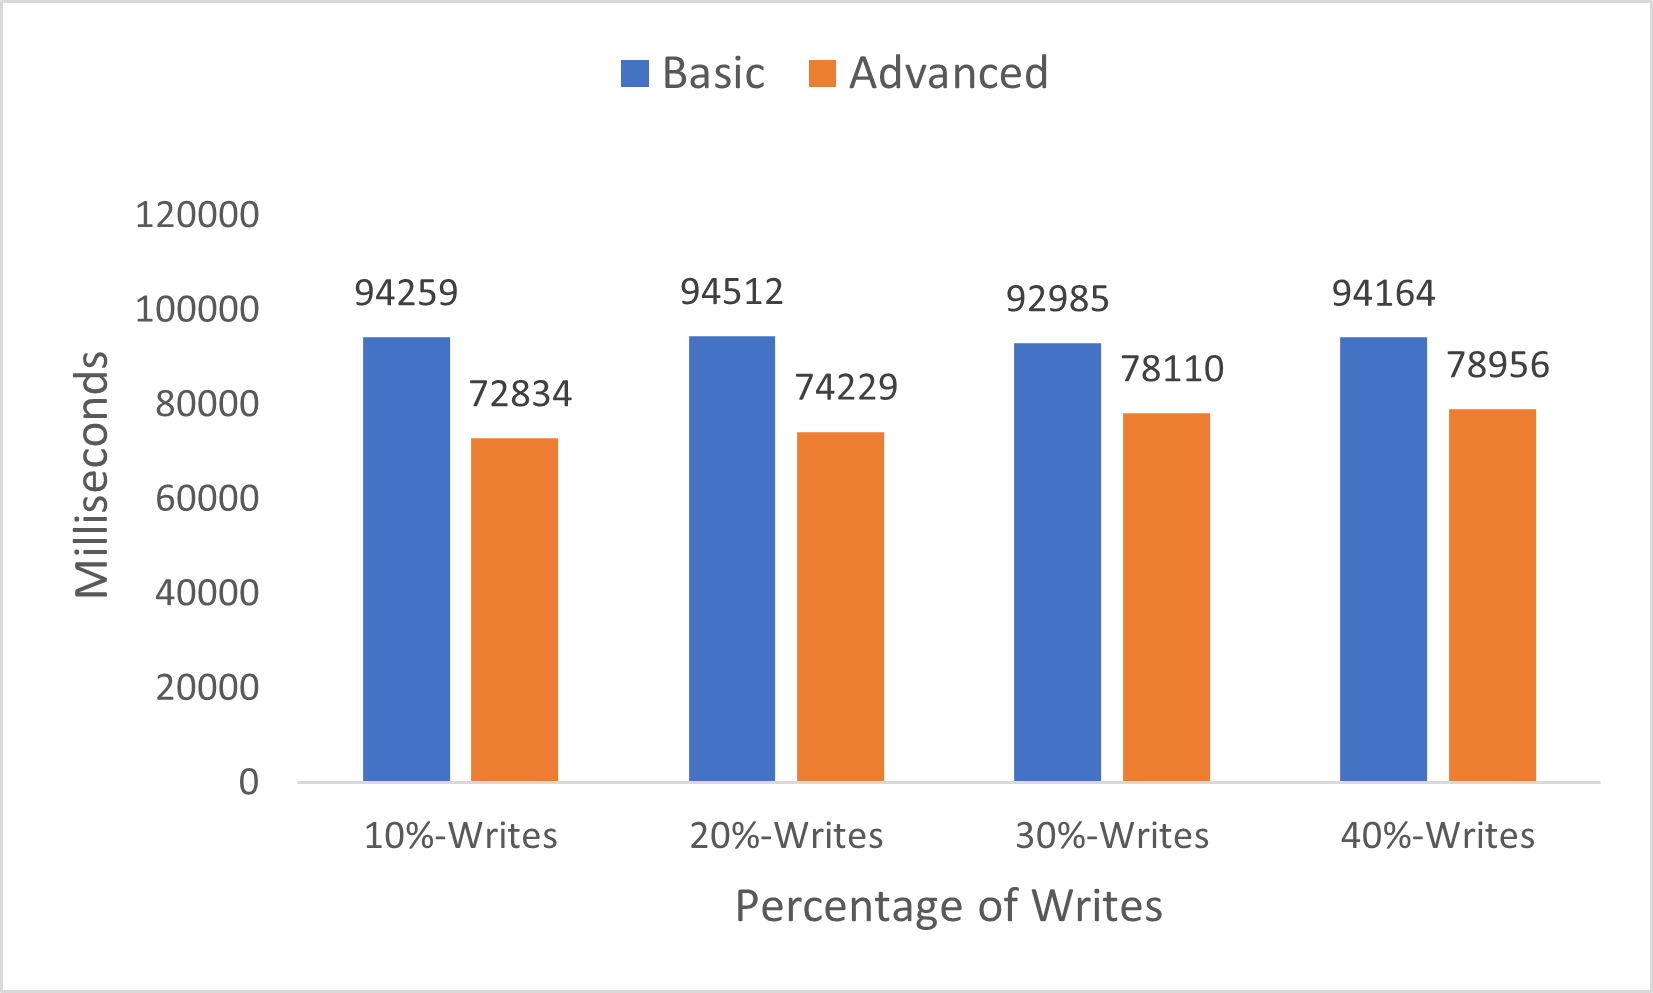
\includegraphics[scale=0.65]{Graphs/Client-10-40.png}
	\caption{Average Time of 10 Clients performing 3000 operations each, on 3 partitions with a total of 10 servers, where 40\% crashed.}
	\vspace{0.15in}
	\centering
	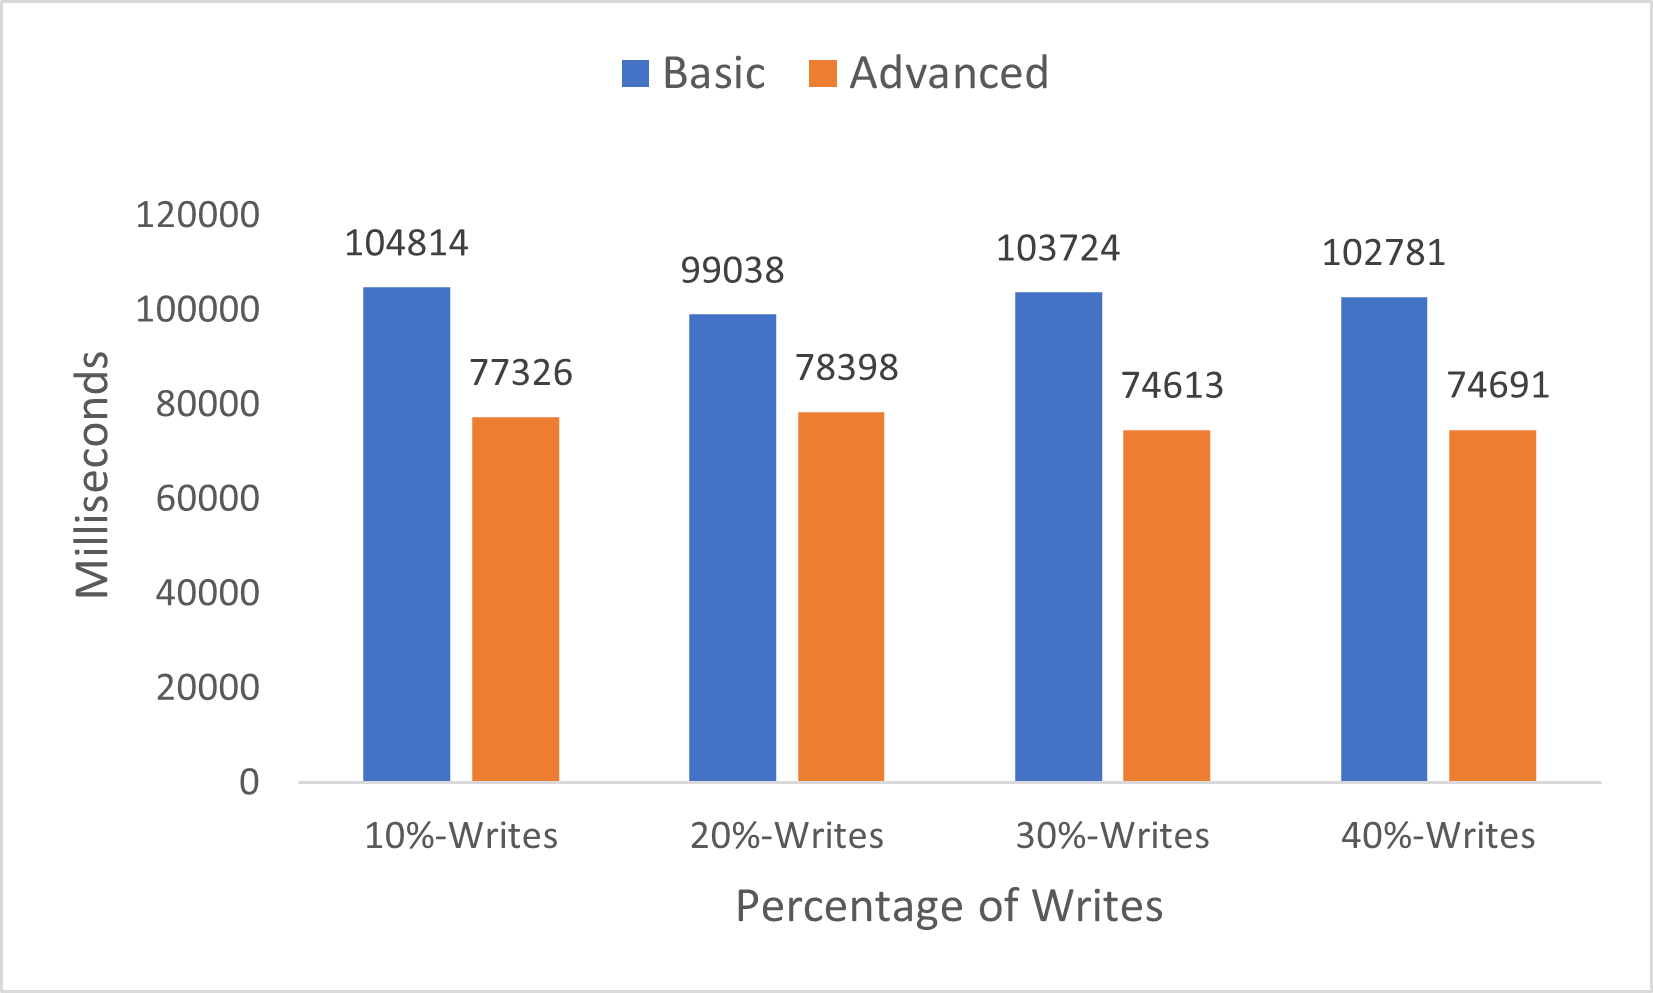
\includegraphics[scale=0.65]{Graphs/Client-10-60.png}
	\caption{Average Time of 10 Clients performing 3000 operations each, on 3 partitions with a total of 10 servers, where 60\% crashed.}
\end{figure}
%------------------------------------------------------------------------- 
\SubSubSection{Discussion of Results}
These graphs illustrate the performance of a system composed by a total of 10 servers on 3 partitions with 6 servers each.

The results are similar to the ones described on the above scenario. This scenario has a larger number of servers in each partition which will lead the \textbf{Basic Version} to be incrementally less efficient when crashes occur, because the perfect failure detector of our system takes time to acknowledge a crash, and as operations need to be fully propagated to all partition servers it will wait for all those acknowledges, which does not happen on the \textbf{Advanced Version} since only a quorum of answers is needed in order to successfully complete an operation.
%------------------------------------------------------------------------- 
\SubSection{Scenario: System with 20 Servers}
\begin{figure}[h!]
	\centering
	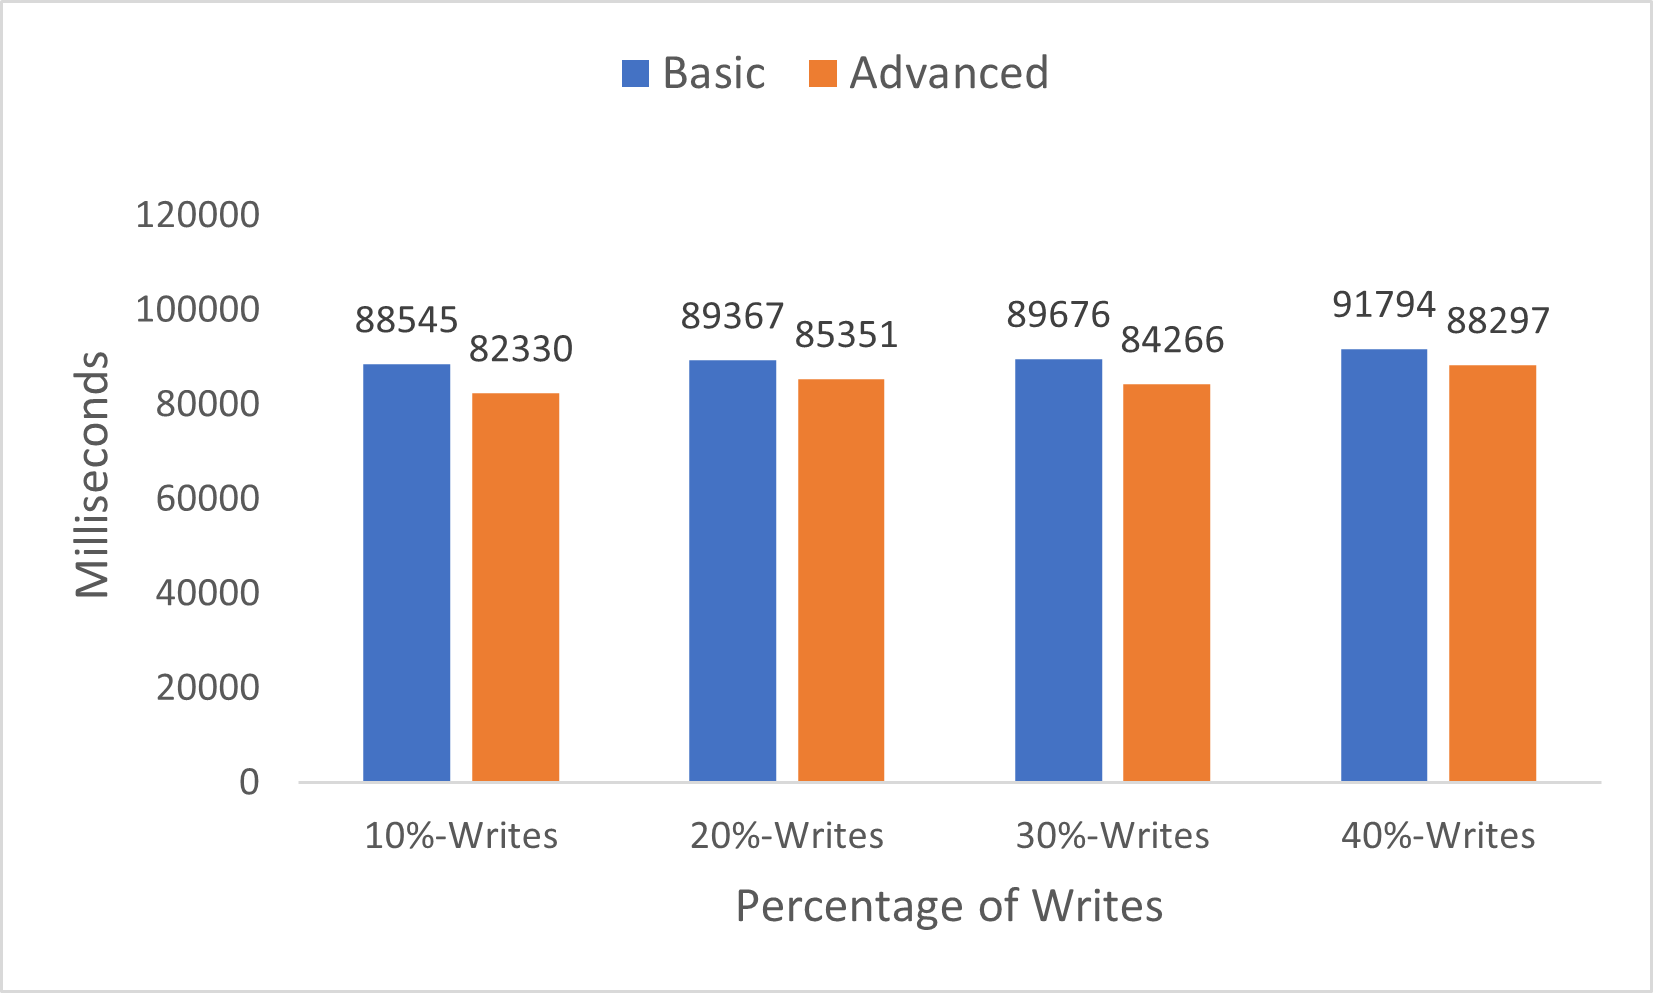
\includegraphics[scale=0.65]{Graphs/Client-20-20.png}
	\caption{Average Time of 10 Clients performing 3000 operations each, on 3 partitions with a total of 20 servers, where 20\% crashed.}
	\vspace{0.15in}
	\centering
	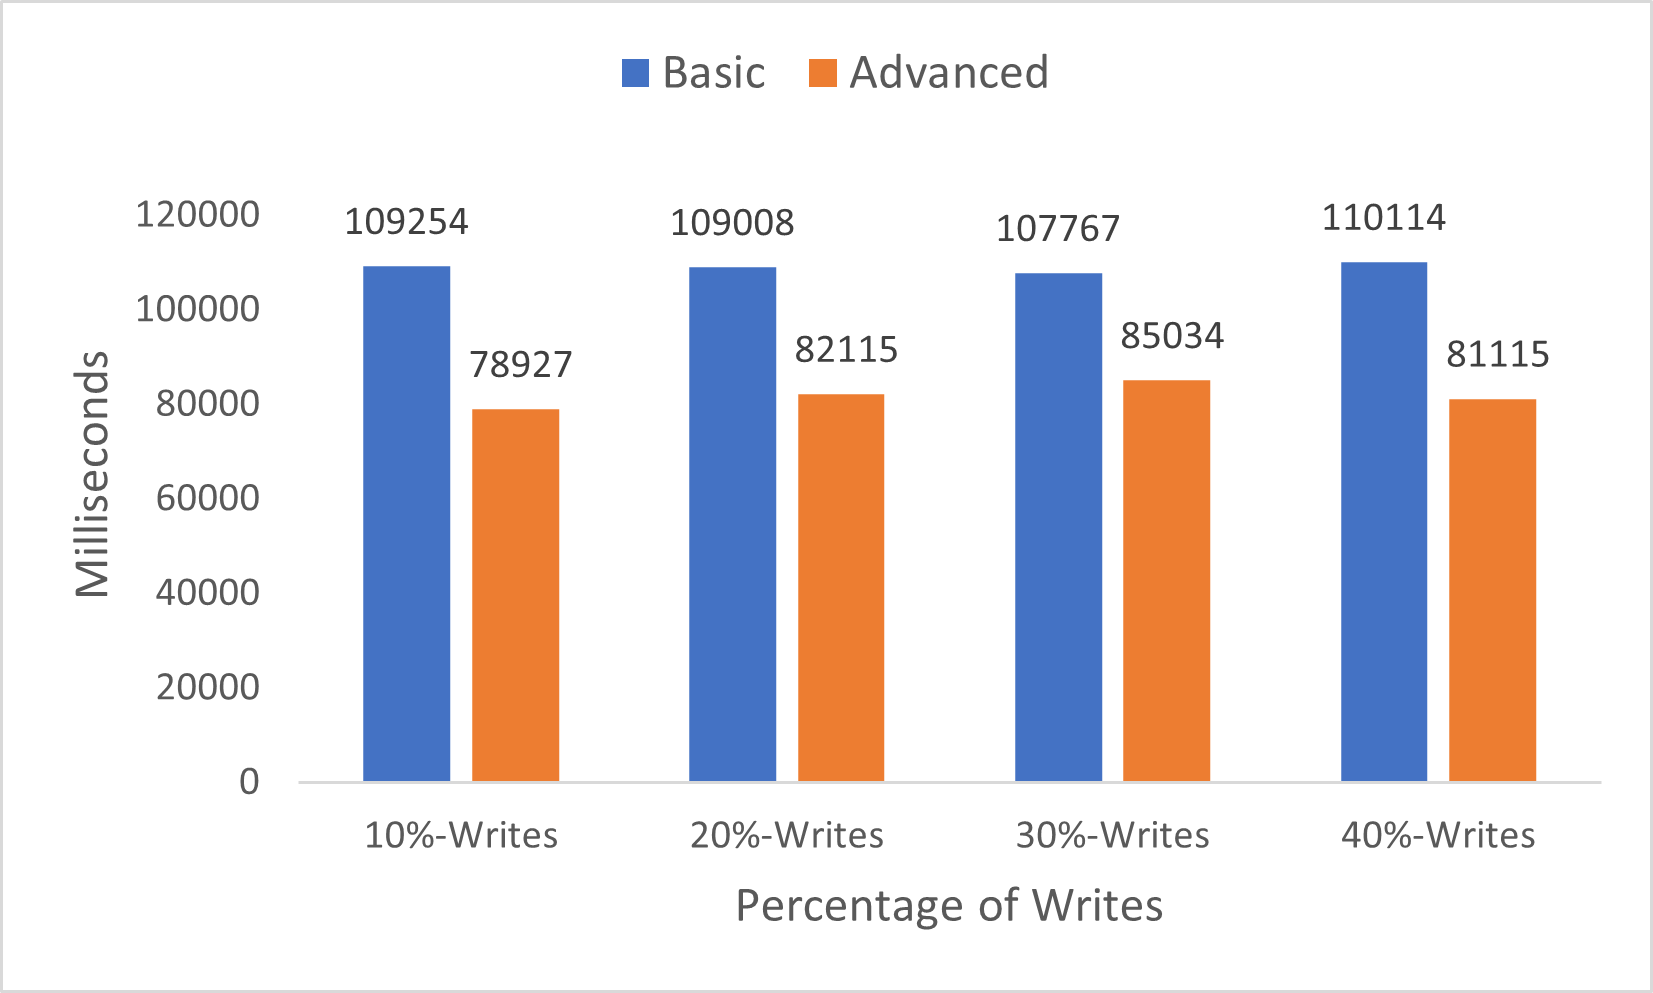
\includegraphics[scale=0.65]{Graphs/Client-20-40.png}
	\caption{Average Time of 10 Clients performing 3000 operations each, on 3 partitions with a total of 20 servers, where 40\% crashed.}
\end{figure}
\newpage
\begin{figure}[h!]
	\centering
	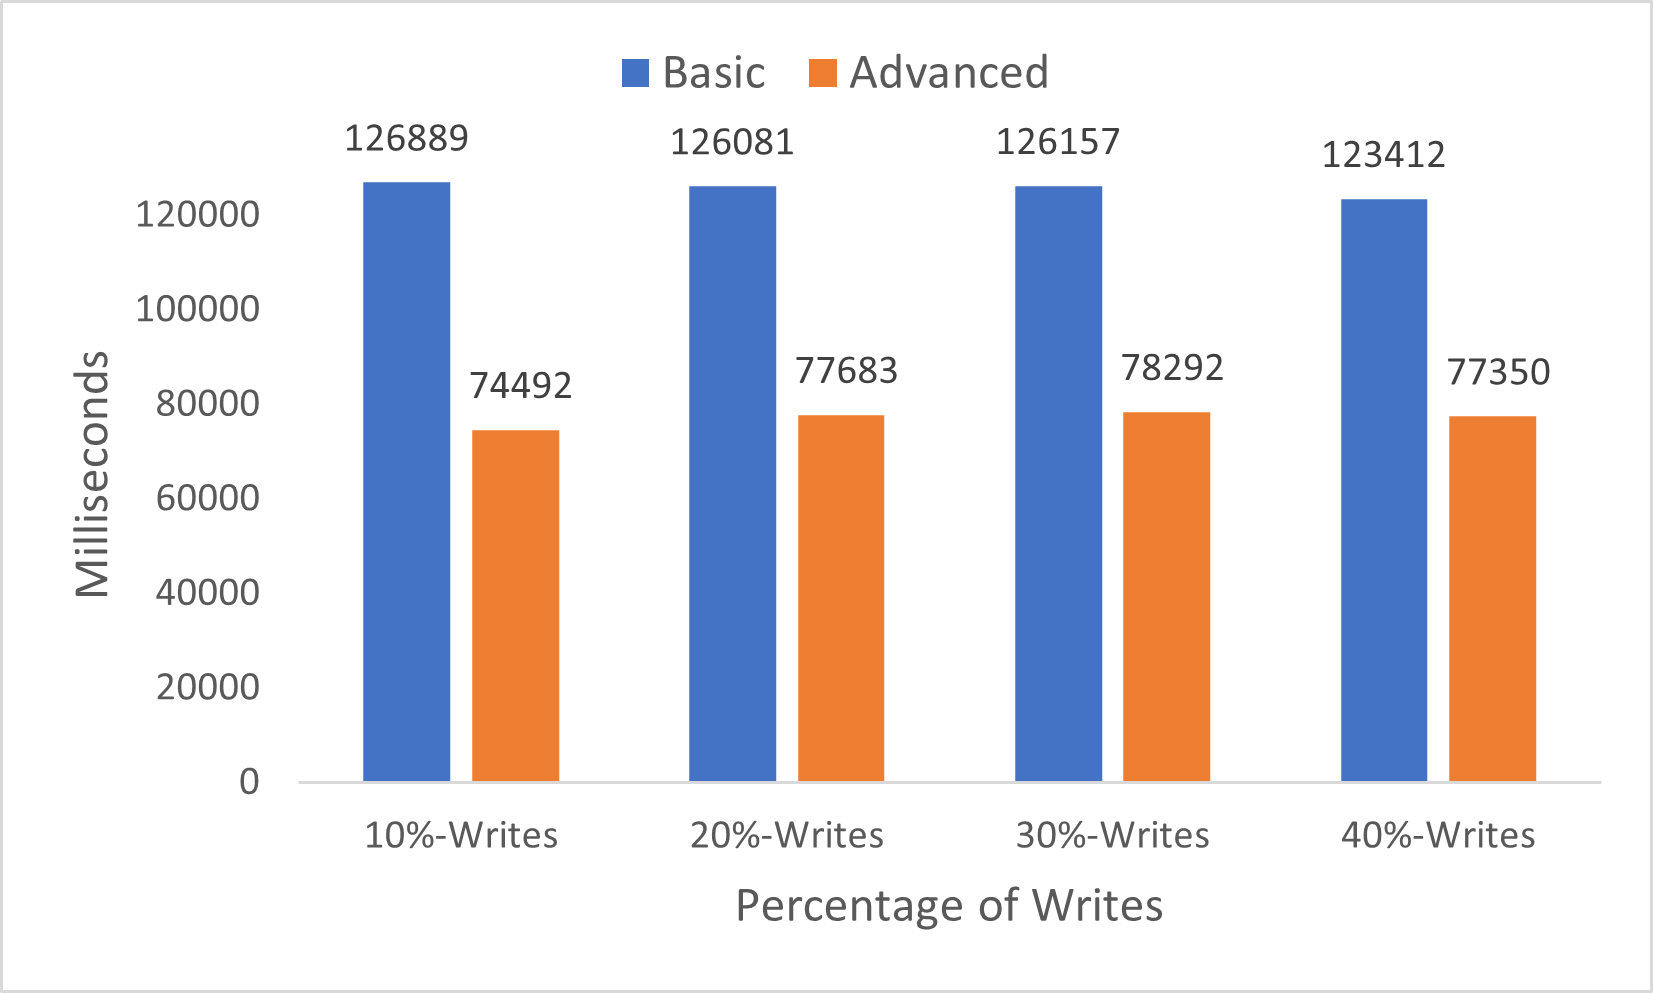
\includegraphics[scale=0.65]{Graphs/Client-20-60.png}
	\caption{Average Time of 10 Clients performing 3000 operations each, on 3 partitions with a total of 20 servers, where 60\% crashed.}
\end{figure}
%------------------------------------------------------------------------- 
\SubSubSection{Discussion of Results}
These graphs illustrate the performance of a system composed by a total of 20 servers on 3 partitions with 12 servers each.

The results are similar to the ones described on both scenarios, and the reason why the difference of performance between the \textbf{Basic Version} and the \textbf{Advanced Version} is more accentuated on each graph is the same as described on the above scenario.
%------------------------------------------------------------------------- 
\SubSection{Scenario: Master is Frozen}
\begin{figure}[h!]
	\centering
	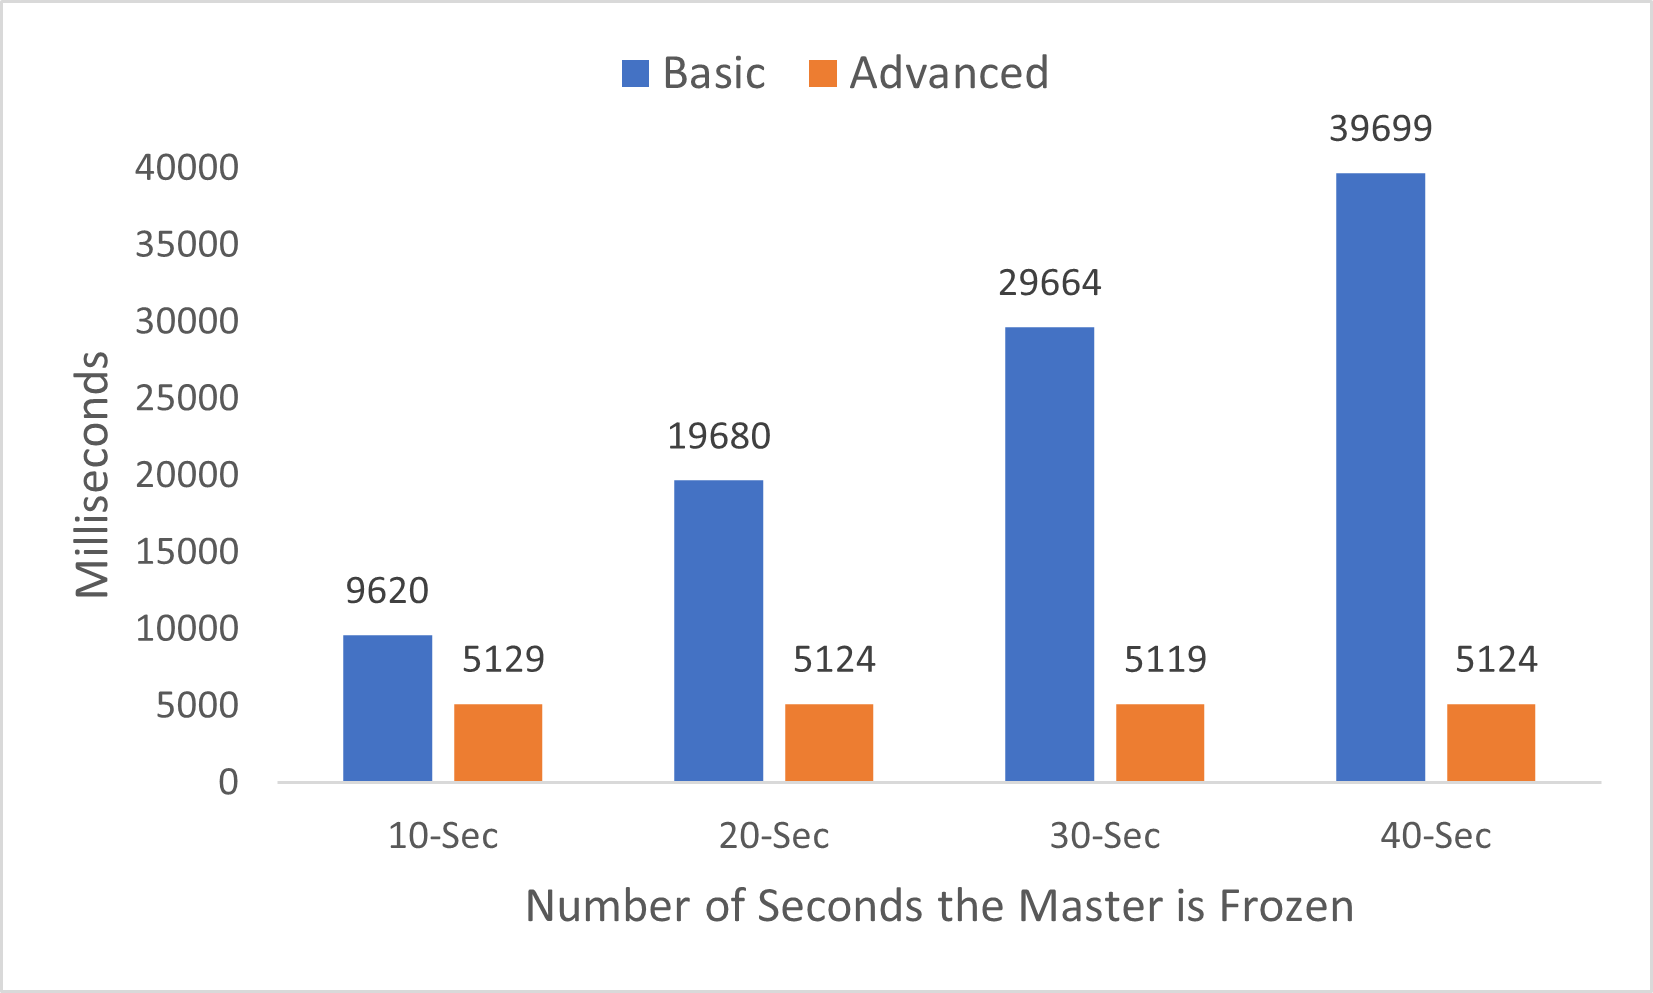
\includegraphics[scale=0.65]{Graphs/Client-FreezeMaster.png}
	\caption{Average Time of 10 Clients performing 1 write each, on 1 partition with a total of 3 servers, where the Master is frozen.}
\end{figure}
\newpage
%------------------------------------------------------------------------- 
\SubSubSection{Discussion of Results}
This graph illustrates the ability of environment adaptation that the \textbf{Advanced Version} offers. On the \textbf{Basic Version} when a Master freezes a client will be blocked until it is unfrozen. On the \textbf{Advanced Version} a new Master will be elected as soon as followers detect the previous Master is unavailable, which will allow a client to continue performing write operations. The client will timeout (5 Seconds) detecting the Master is currently unavailable, and it will try to reach the remaining partition servers, once at a time, in order to find the new Master that can perform its desired request.
%------------------------------------------------------------------------- 
\SubSection{Conclusions}
\textbf{GStore} was a fascinating and complex project. Both requested versions were successfully implemented. The \textbf{Basic Version} was implemented as the statement of the project intended, while in the \textbf{Advanced Version} it was given more freedom to decide how to implement it. The decided approach for the implementation of the \textbf{Advanced Version} of this system was to use the RAFT [1] algorithm, because although it had a more relaxed consistency, it would clearly improve the performance of the previous version and solve the single point of failure problem with its elections. It was decided that the consistency relaxation was not a critical problem in this Key-Value Pair Storage System.
%------------------------------------------------------------------------- 
\nocite{ex1,ex2}
\bibliographystyle{latex8}
\bibliography{latex8}
\end{document}

